\exercisesheader{}

% 1

\eoce{\qt{Mammal life spans\label{mammal_life_spans}} Data were collected on life spans (in 
years) and gestation lengths (in days) for 62 mammals. A scatterplot of life span versus 
length of gestation is shown below. \footfullcite{Allison+Cicchetti:1975}

\noindent\begin{minipage}[c]{0.44\textwidth}
\begin{parts}
\item What type of an association is apparent between life span and length of gestation?
\item What type of an association would you expect to see if the axes of the plot were reversed, i.e. if we plotted length of gestation versus life span?
\item Are life span and length of gestation independent? Explain your reasoning.
\end{parts}
\end{minipage}
\begin{minipage}[c]{0.55\textwidth}
\begin{center}
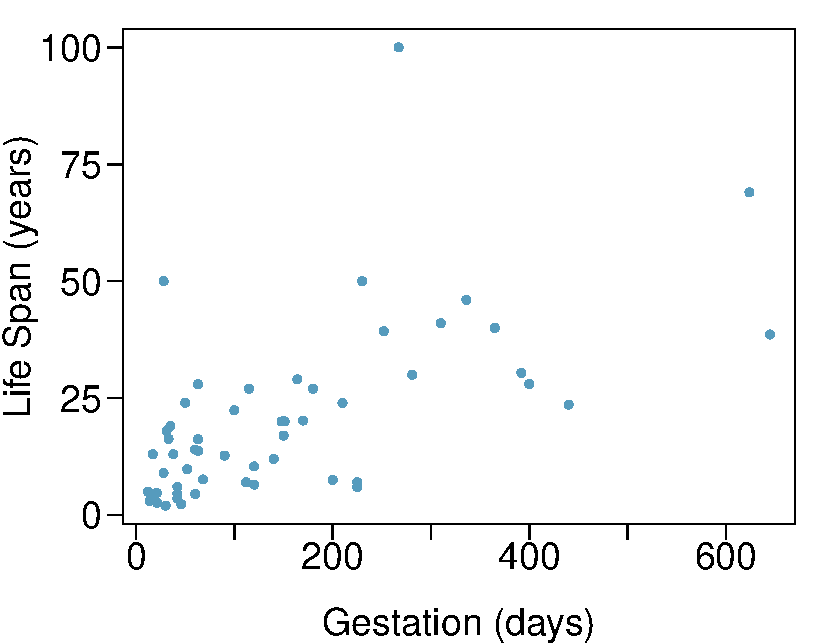
\includegraphics[width = 0.86\textwidth]{ch_summarizing_data/figures/eoce/mammal_life_spans/mammal_life_spans_scatterplot.pdf}
\end{center}
\end{minipage}
}{}

% 2

\eoce{\qt{Associations\label{association_plots}}
Indicate which of the plots show
(a)~a positive association,
(b)~a negative association, or
(c)~no~association.
Also determine if the positive and negative associations
are linear or nonlinear.
Each part may refer to more than one plot.
\begin{center}
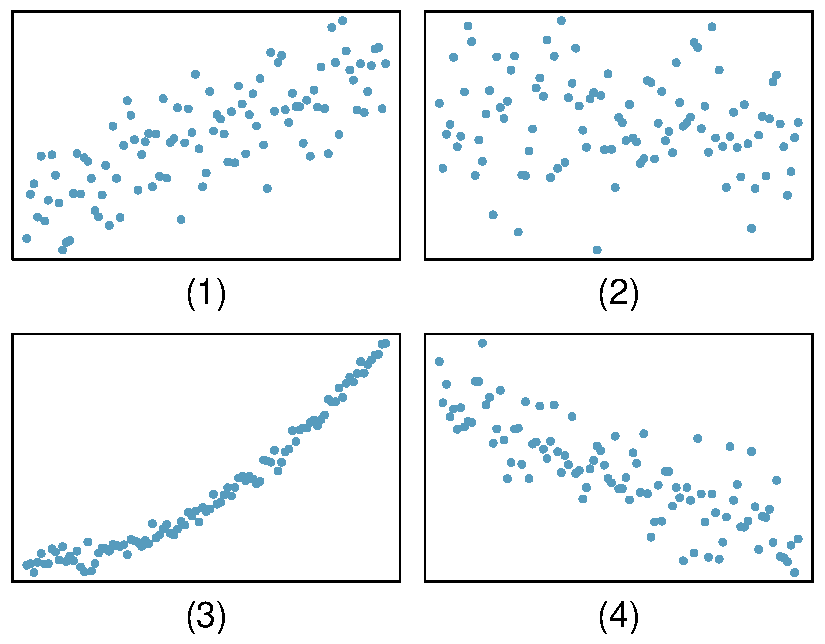
\includegraphics[width = 0.95\textwidth]{ch_summarizing_data/figures/eoce/association_plots/association_plots.pdf}
\end{center}
}{}

% 3

\eoce{\qt{Reproducing bacteria\label{reproducing_bacteria}} Suppose that there is only 
sufficient space and nutrients to support one million bacterial cells in a petri dish. 
You place a few bacterial cells in this petri dish, allow them to reproduce freely, and 
record the number of bacterial cells in the dish over time. Sketch a plot representing 
the relationship between number of bacterial cells and time.
% first exponential
}{}

% 4

\eoce{\qt{Office productivity\label{office_productivity}} Office productivity is relatively low 
when the employees feel no stress about their work or job security. However, high levels 
of stress can also lead to reduced employee productivity. Sketch a plot to represent the 
relationship between stress and productivity.
}{}

% 5

\eoce{\qt{Parameters and statistics\label{parameters_stats}} Identify which value represents 
the sample mean and which value represents the claimed population mean.
\begin{parts}
\item American households spent an average of about \$52 in 2007 on Halloween 
merchandise such as costumes, decorations and candy. To see if this number had changed, 
researchers conducted a new survey in 2008 before industry numbers were reported. The 
survey included 1,500 households and found that average Halloween spending was \$58 per 
household.
\item The average GPA of students in 2001 at a private university was 3.37. A survey 
on a sample of 203 students from this university yielded an average GPA of 3.59 
a decade later.
\end{parts}
}{}

% 6

\eoce{\qt{Sleeping in college\label{college_sleeping}} A recent article in a college newspaper 
stated that college students get an average of 5.5 hrs of sleep each night. A student who 
was skeptical about this value decided to conduct a survey by randomly sampling 25 
students. On average, the sampled students slept 6.25 hours per night. Identify which 
value represents the sample mean and which value represents the claimed population mean.
}{}

% 7

\eoce{\qt{Days off at a mining plant\label{days_off_mining}} Workers at a particular mining 
site receive an average of 35 days paid vacation, which is lower than the national 
average. The manager of this plant is under pressure from a local union to increase the 
amount of paid time off. However, he does not want to give more days off to the workers 
because that would be costly. Instead he decides he should fire 10 employees in such a 
way as to raise the average number of days off that are reported by his employees. In 
order to achieve this goal, should he fire employees who have the most number of days 
off, least number of days off, or those who have about the average number of days off?
}{}

% 8

\eoce{\qt{Medians and IQRs} For each part, compare distributions (1) and (2) based on their medians and IQRs. You do not need to calculate these statistics; simply state how the medians and IQRs compare. Make sure to explain your reasoning. 
\begin{multicols}{2}
\begin{parts}
\item (1) 3, 5, 6, 7, 9 \\
(2) 3, 5, 6, 7, 20
\item (1) 3, 5, 6, 7, 9 \\
(2) 3, 5, 7, 8, 9
\item (1) 1, 2, 3, 4, 5 \\
(2) 6, 7, 8, 9, 10
\item (1) 0, 10, 50, 60, 100 \\
(2) 0, 100, 500, 600, 1000
\end{parts}
\end{multicols}
}{}

% 9

\eoce{\qt{Means and SDs} For each part, compare distributions (1) and (2) based on their means and standard deviations. You do not need to calculate these statistics; simply state how the means and the standard deviations compare. Make sure to explain your reasoning. \textit{Hint:} It may be useful to sketch dot plots of the distributions.
\begin{multicols}{2}
\begin{parts}
\item (1) 3, 5, 5, 5, 8, 11, 11, 11, 13 \\
(2) 3, 5, 5, 5, 8, 11, 11, 11, 20 \\
\item (1) -20, 0, 0, 0, 15, 25, 30, 30 \\
(2) -40, 0, 0, 0, 15, 25, 30, 30
\item (1) 0, 2, 4, 6, 8, 10 \\
(2) 20, 22, 24, 26, 28, 30
\item (1) 100, 200, 300, 400, 500 \\
(2) 0, 50, 300, 550, 600
\end{parts}
\end{multicols}
}{}

% 10

\eoce{\qt{Mix-and-match} Describe the distribution in the histograms below and match them to the box plots. \\
\begin{center}
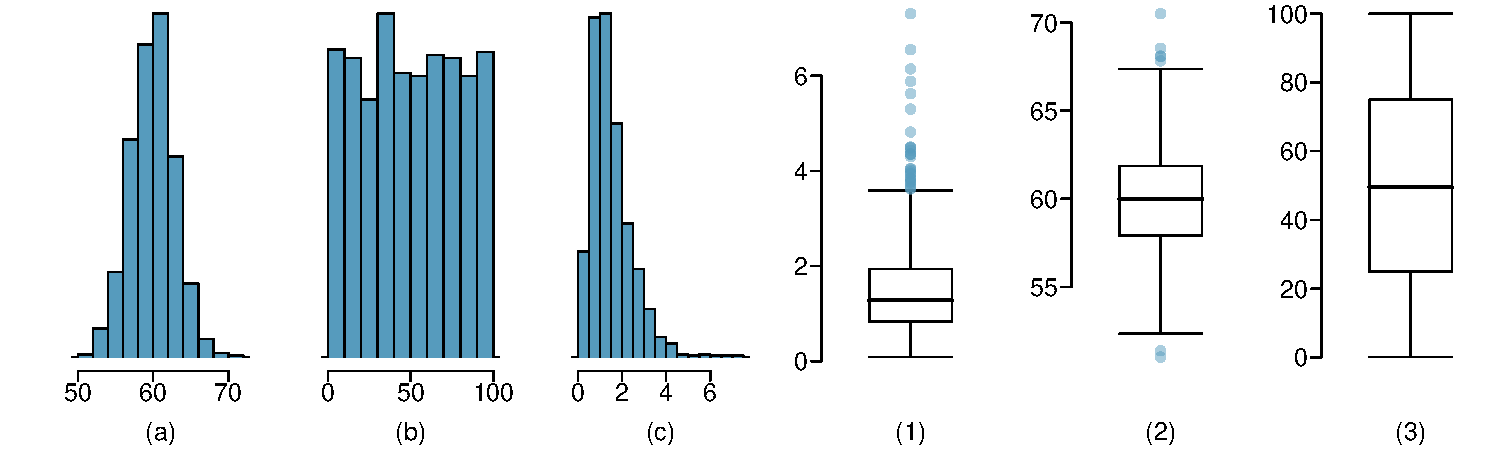
\includegraphics[width=\textwidth]{ch_summarizing_data/figures/eoce/hist_box_match/hist_box_match.pdf}
\end{center}
}{}

% 11

\eoce{\qt{Air quality\label{air_quality_durham}} Daily air quality is measured by the air 
quality index (AQI) reported by the Environmental Protection Agency. This index reports 
the pollution level and what associated health effects might be a concern. The index is 
calculated for five major air pollutants regulated by the Clean Air Act and takes values 
from 0 to 300, where a higher value indicates lower air quality. AQI was reported for a 
sample of 91 days in 2011 in Durham, NC. The relative frequency histogram below shows 
the distribution of the AQI values on these days. \footfullcite{data:durhamAQI:2011} \\
\begin{minipage}[c]{0.55\textwidth}
\begin{parts}
\item Estimate the median AQI value of this sample.
\item Would you expect the mean AQI value of this sample to be higher or lower than the 
median? Explain your reasoning.
\item Estimate Q1, Q3, and IQR for the distribution.
\item Would any of the days in this sample be considered to have an unusually low or 
high AQI? Explain your reasoning.
\end{parts}
\end{minipage}
\begin{minipage}[c]{0.45\textwidth}
\begin{center}
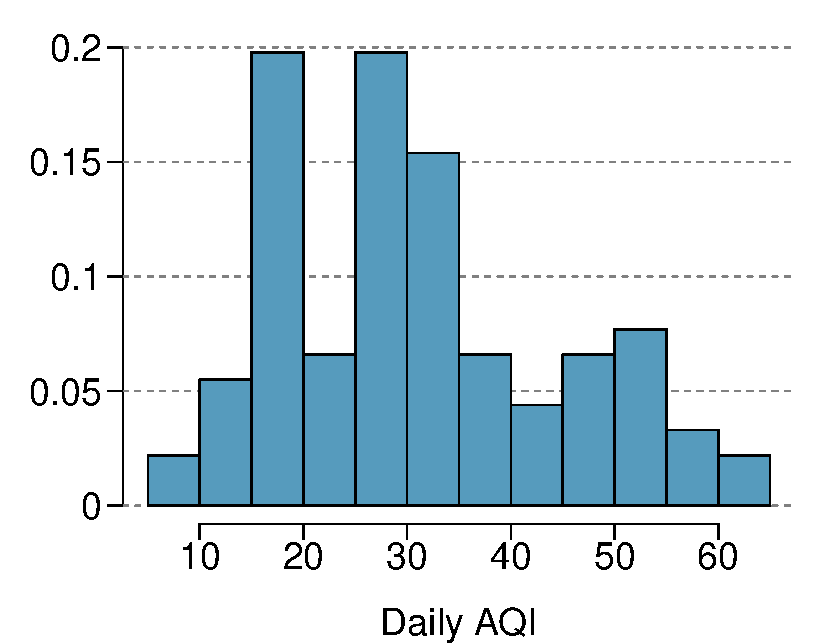
\includegraphics[width = \textwidth]{ch_summarizing_data/figures/eoce/air_quality_durham/air_quality_durham_rel_freq_hist.pdf} 
\end{center}
\end{minipage}
}{}

% 12

\eoce{\qt{Median vs. mean\label{estimate_mean_median_simple}} Estimate the median for the 
400 observations shown in the histogram, and note whether you expect the mean 
to be higher or lower than the median.
\begin{center}
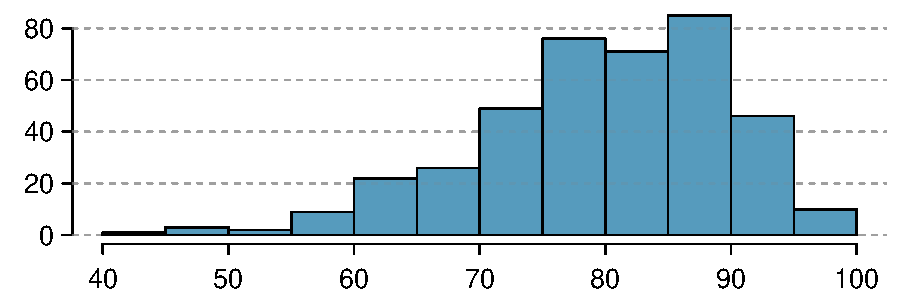
\includegraphics[width = 0.6\textwidth]{ch_summarizing_data/figures/eoce/estimate_mean_median_simple/estimate_mean_median_simple.pdf} 
\end{center}
}{}

% 13

\eoce{\qt{Histograms vs. box plots\label{hist_vs_box}} Compare the two plots below. What 
characteristics of the distribution are apparent in the histogram and not in the box 
plot? What characteristics are apparent in the box plot but not in the histogram?
\begin{center}
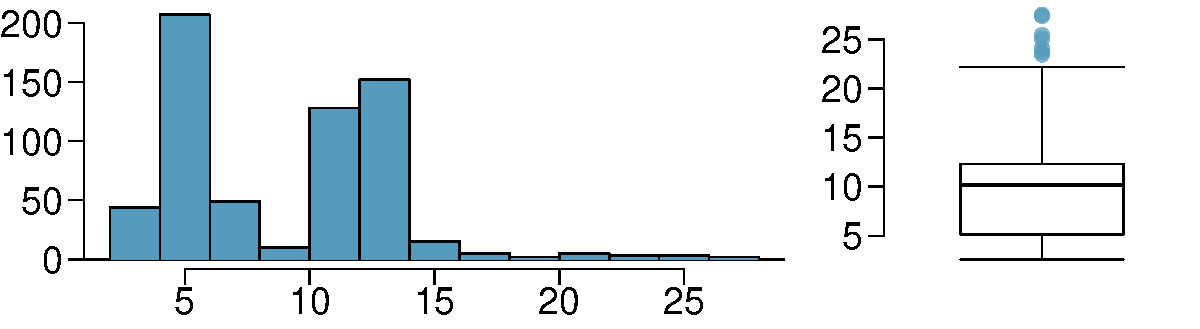
\includegraphics[width = 0.6\textwidth]{ch_summarizing_data/figures/eoce/hist_vs_box/hist_vs_box.pdf}
\end{center}
}{}

% 14

\eoce{\qt{Facebook friends\label{dist_shape_fb_friends}} Facebook data indicate that 
50\% of Facebook users have 100 or more friends, and that the average friend 
count of users is 190. What do these findings suggest about the shape of the 
distribution of number of friends of Facebook users? \footfullcite{Backstrom:2011}
}{}

% 15

\eoce{\qt{Distributions and appropriate statistics, Part I\label{dist_shape_pets_dist_height}} 
For each of the following, state whether you expect the distribution to be 
symmetric, right skewed, or left skewed. Also specify whether the mean or 
median would best represent a typical observation in the data, and whether 
the variability of observations would be best represented using the 
standard deviation or IQR. Explain your reasoning.
\begin{parts}
\item Number of pets per household. 
\item Distance to work, i.e. number of miles between work and home.
\item Heights of adult males.
\end{parts}
}{}

% 16

\eoce{\qt{Distributions and appropriate statistics, Part II\label{dist_shape_housing_alcohol_salary}} 
For each of the following, state whether you expect the distribution to be symmetric, 
right skewed, or left skewed. Also specify whether the mean or median would best 
represent a typical observation in the data, and whether the variability of observations 
would be best represented using the standard deviation or IQR. Explain your reasoning.
\begin{parts}
\item Housing prices in a country where 25\% of the houses cost below \$350,000, 
50\% of the houses cost below \$450,000, 75\% of the houses cost below \$1,000,000 
and there are a meaningful number of houses that cost more than \$6,000,000.
\item Housing prices in a country where 25\% of the houses cost below \$300,000, 
50\% of the houses cost below \$600,000, 75\% of the houses cost below \$900,000 
and very few houses that cost more than \$1,200,000.
\item Number of alcoholic drinks consumed by college students in a given week. 
Assume that most of these students don't drink since they are under 21 years old, 
and only a few drink excessively.
\item Annual salaries of the employees at a Fortune 500 company where only a few 
high level executives earn much higher salaries than all the other employees.
\end{parts}
}{}

% 17

\eoce{\qt{Income at the coffee shop\label{income_coffee_shop}} The first histogram 
below shows the distribution of the yearly incomes of 40 patrons at a college 
coffee shop. Suppose two new people walk into the coffee shop: one making 
\$225,000 and the other \$250,000. The second histogram shows the new income 
distribution. Summary statistics are also provided. \\
\begin{minipage}[c]{0.57\textwidth}
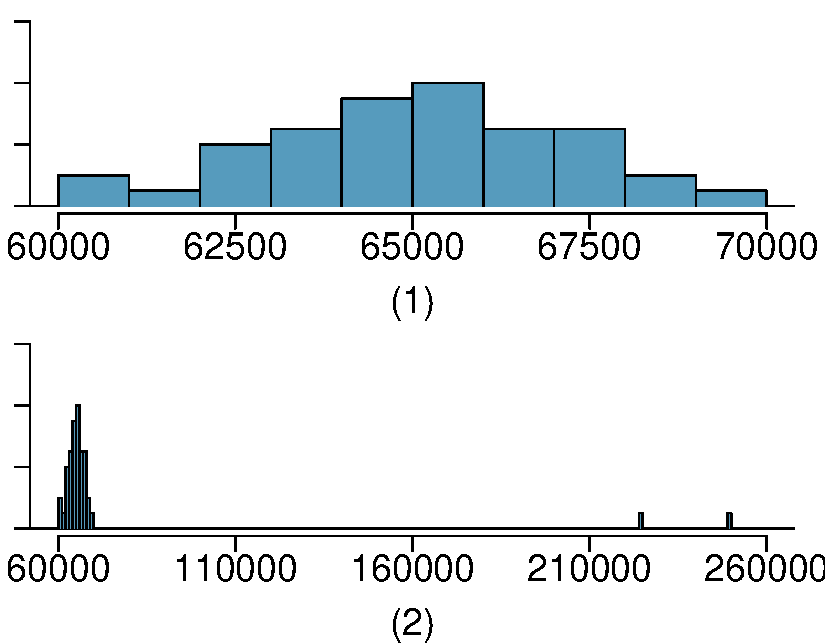
\includegraphics[width=\textwidth]{ch_summarizing_data/figures/eoce/income_coffee_shop/income_coffee_shop.pdf}
\end{minipage}
\begin{minipage}[c]{0.4\textwidth}
\begin{center}
\begin{tabular}{rrr}
\hline
        & (1)       & (2) \\ 
\hline
n       & 40        & 42 \\ 
Min.    & 60,680    & 60,680 \\ 
1st Qu. & 63,620    & 63,710 \\ 
Median  & 65,240    & 65,350 \\ 
Mean    & 65,090    & 73,300 \\ 
3rd Qu. & 66,160    & 66,540 \\ 
Max.    & 69,890    & 250,000 \\ 
SD      & 2,122     & 37,321 \\ 
\hline
\end{tabular}
\end{center}
\end{minipage}
\begin{parts}
\item Would the mean or the median best represent what we might think of as a 
typical income for the 42 patrons at this coffee shop? What does this say about 
the robustness of the two measures?
\item Would the standard deviation or the IQR best represent the amount of 
variability in the incomes of the 42 patrons at this coffee shop? What does 
this say about the robustness of the two measures?
\end{parts}
}{}

% 18

\eoce{\qt{Midrange\label{midrange}} The \textit{midrange} of a distribution is defined as 
the average of the maximum and the minimum of that distribution. Is this statistic 
robust to outliers and extreme skew? Explain your reasoning
}{}

% 19

\eoce{\qt{Commute times\label{county_commute_times}} The US census collects data on 
time it takes Americans to commute to work, among many other variables. The 
histogram below shows the distribution of average commute times in 3,142 US 
counties in 2010. Also shown below is a spatial intensity map of the same data.
\begin{center}
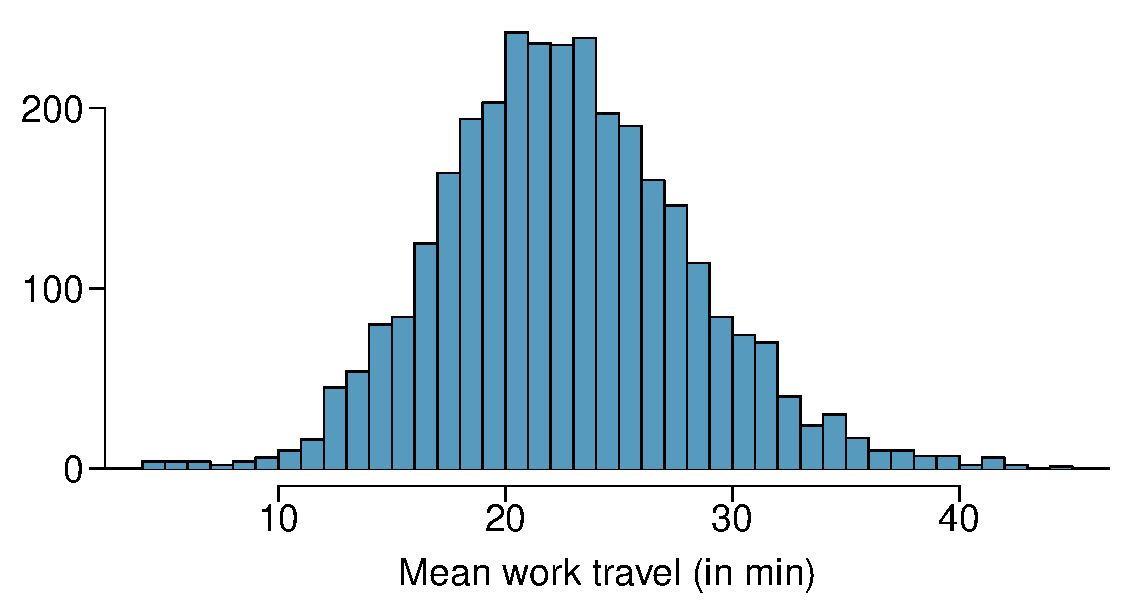
\includegraphics[width=0.48\textwidth]{ch_summarizing_data/figures/eoce/county_commute_times/county_commute_times_hist.pdf}
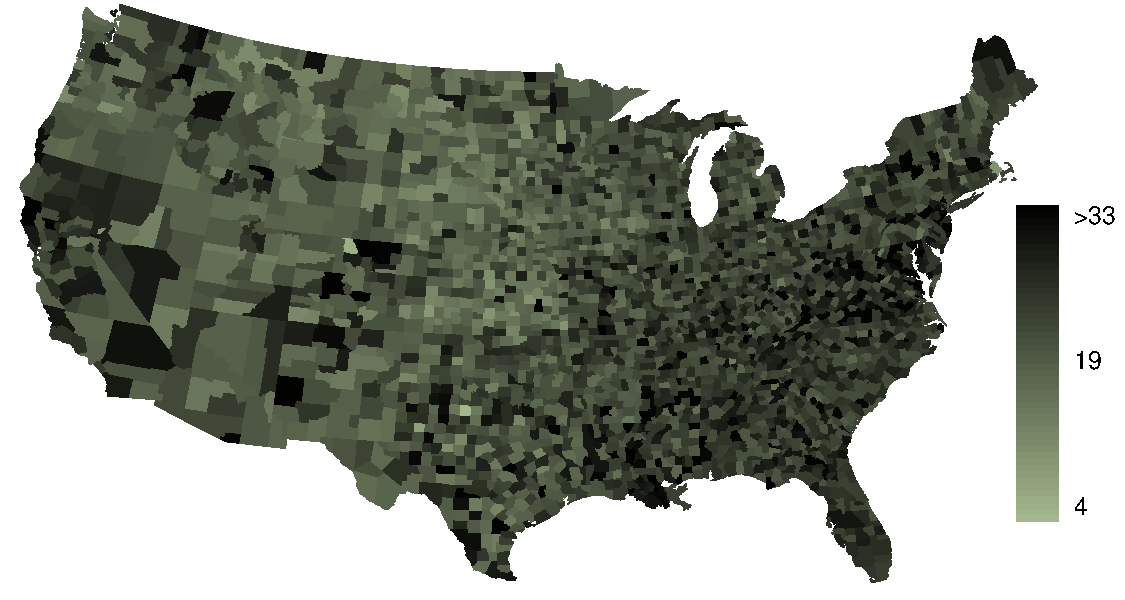
\includegraphics[width=0.48\textwidth]{ch_summarizing_data/figures/eoce/county_commute_times/county_commute_times_map.pdf}
\end{center}
\begin{parts}
\item Describe the numerical distribution and comment on whether or not a log 
transformation may be advisable for these data.
\item Describe the spatial distribution of commuting times using the map below.
\end{parts} 
}{}

% 20

\eoce{\qt{Hispanic population\label{county_hispanic_pop}} The US census collects 
data on race and ethnicity of Americans, among many other variables. The 
histogram below shows the distribution of the percentage of the population 
that is Hispanic in 3,142 counties in the US in 2010. Also shown is a 
histogram of logs of these values.
\begin{center}
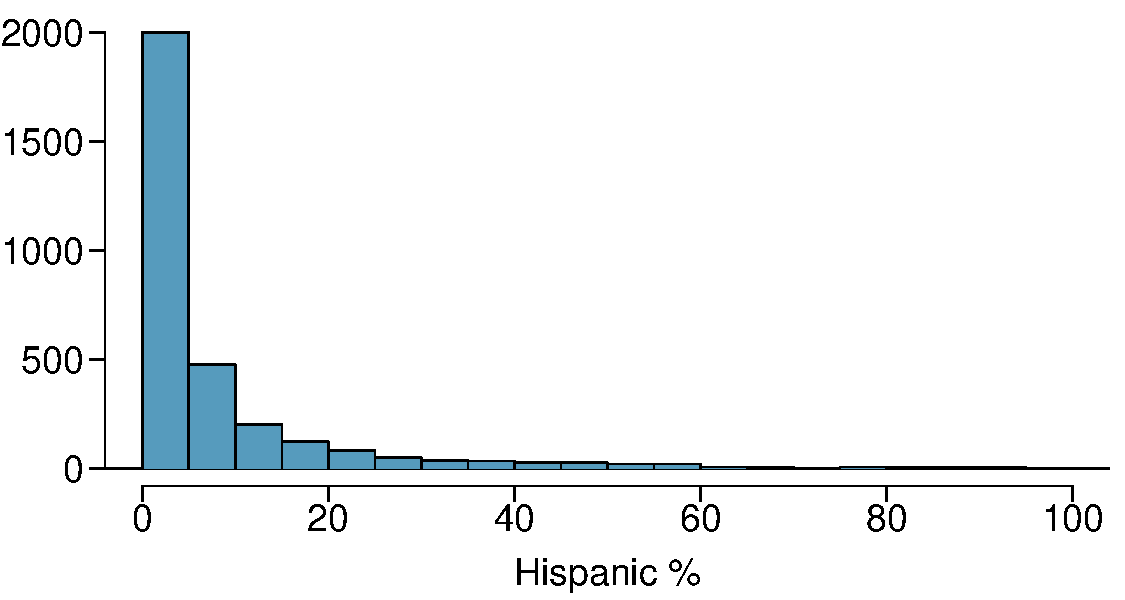
\includegraphics[width=0.48\textwidth]{ch_summarizing_data/figures/eoce/county_hispanic_pop/county_hispanic_pop_hist.pdf}
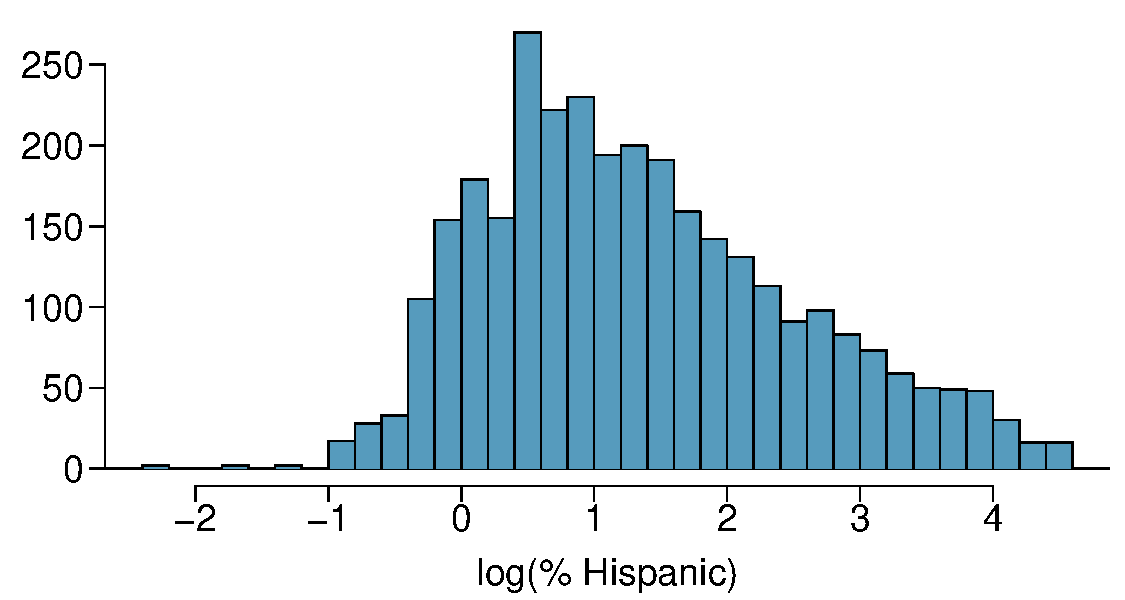
\includegraphics[width=0.48\textwidth]{ch_summarizing_data/figures/eoce/county_hispanic_pop/county_hispanic_pop_log_hist.pdf}
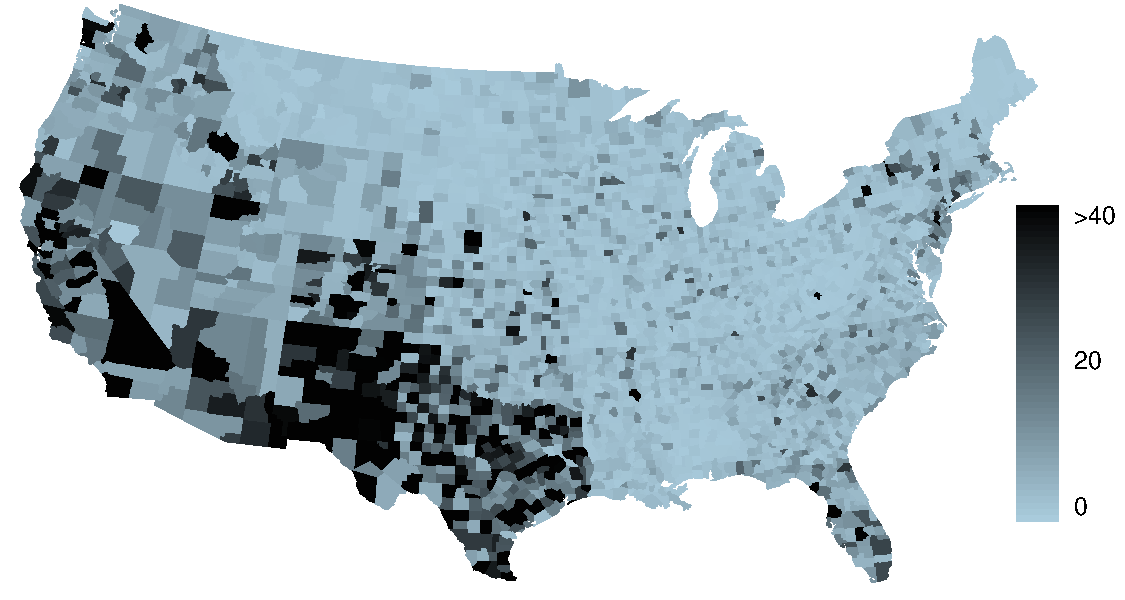
\includegraphics[width=0.48\textwidth]{ch_summarizing_data/figures/eoce/county_hispanic_pop/county_hispanic_pop_map.pdf}
\end{center}
\begin{parts}
\item Describe the numerical distribution and comment on why we might want 
to use log-transformed values in analyzing or modeling these data.
\item What features of the distribution of the Hispanic population in US 
counties are apparent in the map but not in the histogram? What features are 
apparent in the histogram but not the map?
\item Is one visualization more appropriate or helpful than the other? Explain 
your reasoning.
\end{parts} 
}{}
